%----------------------------------------------------------------------------------------
% Define some commands to keep the formatting separated from the content 
\newcommand{\keyword}[1]{\textbf{#1}}
\newcommand{\tabhead}[1]{\textbf{#1}}
\newcommand{\code}[1]{\texttt{#1}}
\newcommand{\file}[1]{\texttt{\bfseries#1}}
\newcommand{\option}[1]{\texttt{\itshape#1}}
%----------------------------------------------------------------------------------------
\chapter{Introduction}
\section{Motivation and background}
Interactions of liquid jets have invoked the curiosity of researchers with their ubiquitous presence, eminent even in the scientific artworks by \cite{da1954notebooks}. The theoretical and experimental analysis accounting for different types of interactions involving liquid jets is classically summarized in a recent effort by \cite{eggers2008physics}. Most elemental among these interactions is the collision between liquid jets which is one of the canonical configurations for generation of liquid sheets. This gives way to atomized droplets in high inertial regime. If the strengths of the two jets are identical, the liquid sheet is formed in the median plane, ie., mid-way between the jets at the point of collision.  \citep{bush2004collision}. This configuration is usually employed in the afterburners of the aircraft or in the thrust engines used in rockets \citep{chen2013high} and has advantages over the conventional coaxial liquid-gas jet atomization technique because of the improved inertial driven destabilization and mixing between jets \citep{erni2013free}. Moreover, the droplets formed in this process come from the thin sheet, making the droplet size distribution skewed towards the lower size and more evenly spread \citep{inoue2008study,inoue2009liquid} as compared to the droplets formed from the single jet atomization as the latter are ejected from a thick liquid jet core instead of a thin sheet. This aids in the post-atomization combustion process \citep{lhuissier2011destabilization}. The collision of laminar jets to form stable sheets is the fundamental case of such atomization processes and also holds physical significance for the exploration of physics behind atomization. Moreover, these structures can be used as wall-free continuous reactors \citep{erni2013free} as well. At low velocities or narrow angles of impingement, jets may coalesce to form a unified one or they may bounce off due to the presence of a thin film of air between them \citep{wadhwa2013noncoalescence}. On increasing the flow rates, laminar jets may lead to the formation of a stable liquid sheet bounded by the thicker rims at the periphery \citep{yang2014liquid}. The inertial and the gravitational forces act to expand the liquid sheet formed, but the action of surface tension helps the sheet to converge so that the successive collisions of the thick rims downstream of the flow result in the formation of mutually orthogonal liquid sheets \citep{bush2004collision}. Figure~\ref{Figure::schematic}(a) illustrates this structure termed as the liquid chain with the complementary orthogonal sheets forming the different links. 
\section{Literature Survey}
\cite{rayleigh1879capillary,rayleigh1889tension} was probably the first researcher to formally study the chain like structures. He reported that the chain structure was generated because of the undulations formed at the surface of a single elliptical liquid jet. Unlike cylindrical jets, they do not have an axis of overall symmetry. This results in thickening of the jet at the periphery leading to the formation of the chain like structure due to collision of these rims.\\
\cite{taylor1960formation} formulated an impingement theory for impact of liquid jets to form a fluid sheet at the median plane, mid-way between the jets. Prior to his work, only the inertial and gravitational forces were considered to describe the phenomenon which gave an expanding liquid sheet. He realized that the flow inside the thicker rim at the periphery can be sustained only if the  surface tension force provides the necessary centripetal acceleration to the fluid parcels inside the rim. The velocity field in the rim is also accelerating due to loss of gravitational potential. On balancing the inertial and surface tension forces, \cite{taylor1960formation} proposed an expression for the sheet radius, given by $r_{max} = \rho u_0Q(\theta)/(2\sigma)$ (where, $u_0$ denotes the average sheet velocity assumed constant throughout including the rim, $Q(\theta)$ implies liquid flux distribution inside the sheet and $\rho$, $\sigma$ are the fluid density and its surface tension coefficient with the air respectively).\\
\cite{bush2004collision} worked on the classical formulation proposed by \cite{taylor1960formation} and gave a comprehensive theoretical and experimental theory for collision of liquid jets. They introduced several regimes to characterize the different flow structures obtained from such collisions and gave an exhaustive experimental analysis of the stable liquid chain formed by the collision of laminar jets. Their work also verifies the formulation given by \cite{taylor1960formation} which predicts the sheet dimensions within experimental precision. Emphasis has been also given by \cite{bush2004collision} for prediction of shapes of leaf-like links forming chain structure. We have used the results developed by them to validate our numerical model.\\
\cite{ibrahim1991impinging} demonstrated that the stable sheet structures can serve as the base case for the atomization studies because the droplets are formed from the perturbed liquid sheet. At high viscosities, different flow instabilities die down but at higher inertial strengths, as the flow becomes turbulent, the flapping atomization takes place.\\
\cite{bremond2006atomization} studied the several instabilities modes related to the rim at the periphery of the sheet. These instabilities are magnified as the velocity of fluid parcels inside the rims increase and the curvature dependent surface tension forces are not able to maintain equilibrium. First, finger like projections are observed at the rims' outer boundaries causing Plateau-Rayleigh instability and droplet generation.\\
\cite{clanet2002life,villermaux2002life} discussed the instabilities inside the liquid sheet. As the velocity exceeds a critical value, the Kelvin-Helmholtz instability takes over and results in formation of destabilizing waves. This also speeds up the process of fingering instabilities at the peripheral rim of the sheet.\\
\cite{choo2001parametric,choo2002velocity,choo2007effect} have worked extensively on the characterization of the first link of the chain structure, including the velocity field inside. Contrary to the earlier belief, they have shown that the sheet velocity is not a constant parameter but varies with the azimuthal angle variation. This has been demonstrated in our studies as well. Moreover, they have also discussed the variation in the sheet characteristics with respect to the velocity profile at the exit of the nozzles, inside the jets. They prescribe a parabolic profile gives a better estimate for the fully developed laminar jet as compared to the uniform profile or any other power law fit. Further, they gave the justification for the presence of thicker liquid rim at the periphery using Particle Image Velocimetry (PIV) technique. The radial streamlines were observed near the point of impingement and the fluid parcels travel towards the periphery resulting in the formation of the thick rim due to fluid accumulation. \\
\cite{inamura2014effect} studied the presence of stagnation point inside the liquid sheet. Unlike the head on collision of liquid jets where this point is at the point of intersection of the jets, it was found to shift upstream by some factor. The factor was found to be dependent on the impingement angle. These works summarize the variation of fluid velocity inside the sheet.\\
\cite{yang2014liquid} discussed the influence of different flow parameters on the shape and size of the first link in the chain structure. They acknowledged the variations due to physical parameters as well. In the present study, their arguments are generalized for the entire chain structure.\\
\cite{chen2013high} have shown the formation of liquid chain using Finite Volume based Volume of Fluid (VOF) framework. They attempted the reproduction of different flow regimes as proposed by \cite{bush2004collision}. The same numerical framework is used in the present method with some modifications on the mesh refinement criteria.\\
\cite{da2016surface} also demonstrated the formation of liquid chain using Boundary Element Method (BEM). This simulation work comprises of inviscid flow assumption but gives mesmerizing fluid structures. They have successfully reproduced all the regimes observed in the experimental works but fail to acknowledge the internal dynamics of the liquid sheet.\\

\begin{figure*}
	\centering
	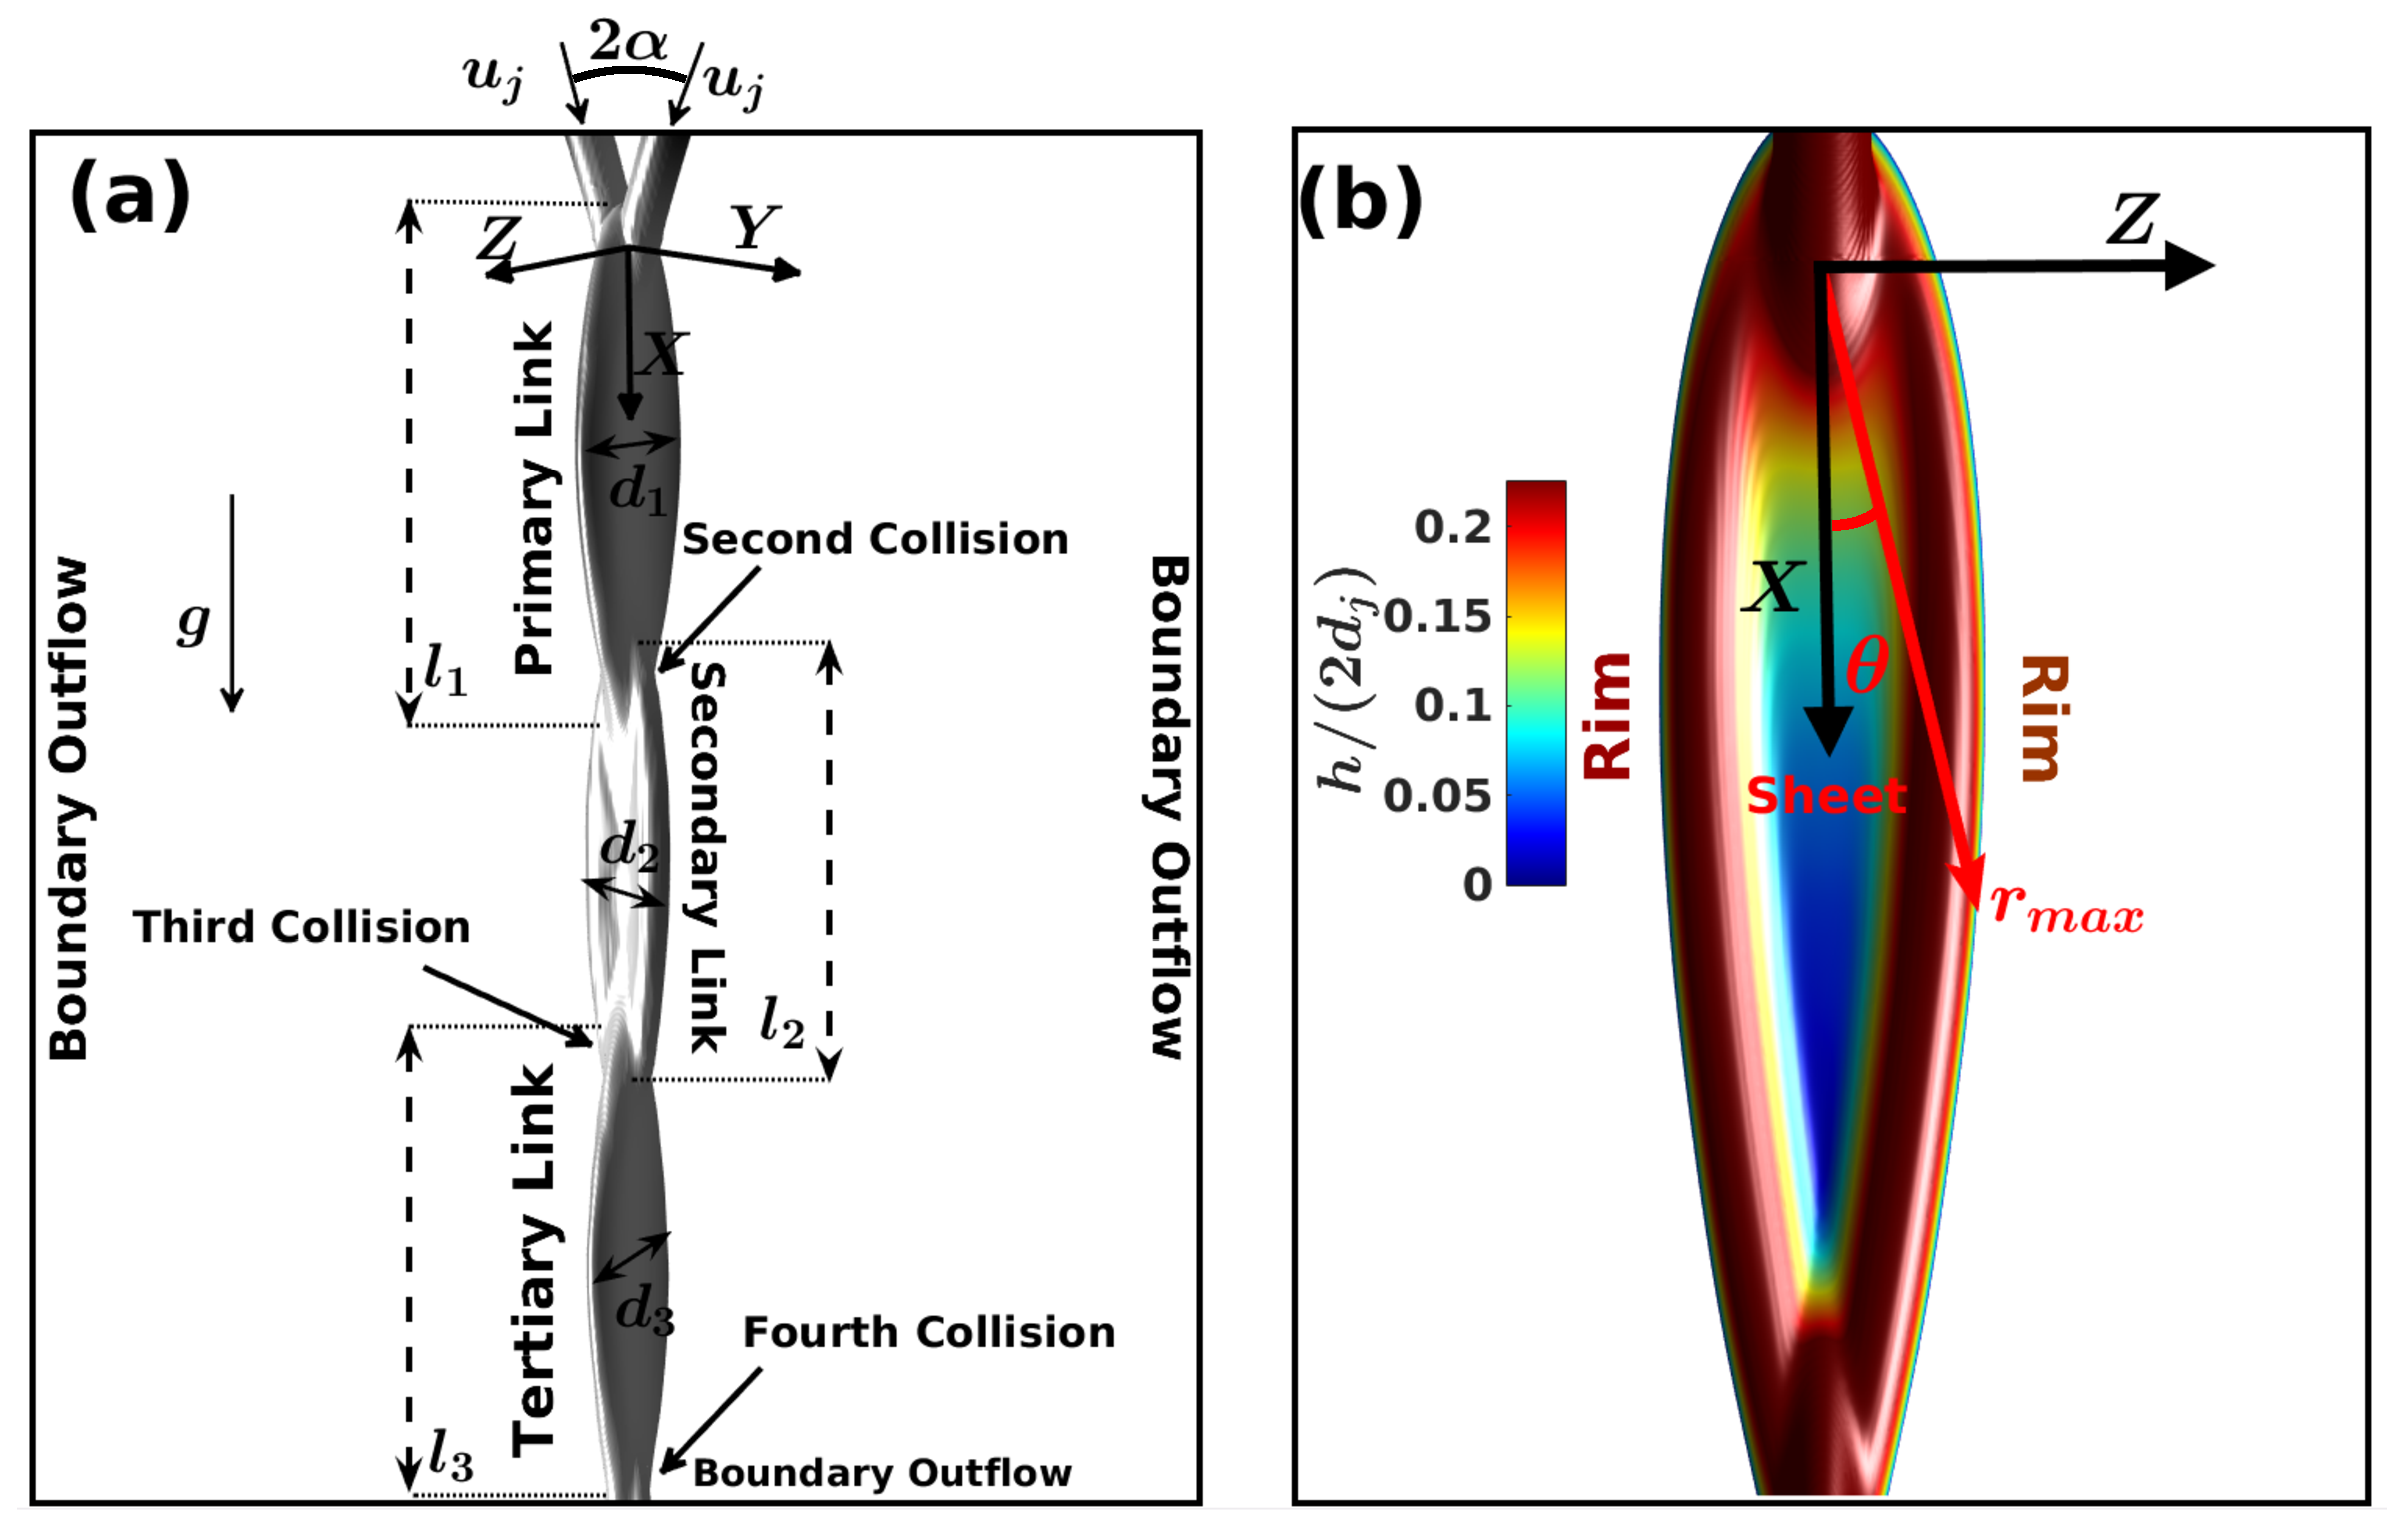
\includegraphics[width=\textwidth]{chapters/Figure1}
	\caption{Formation of the liquid sheet by the collision of laminar jets. (a) Different structural features and length scales. (b) The primary link structure colored based on half times the magnitude of the sheet thickness, non-dimensionalized with the jet diameter $\left(\frac{h}{2d_j}\right)$.}
	\label{Figure::schematic}
\end{figure*}
\section{Lacuna in literature}
Critical assessment of literature reveals that an in-depth study of fluid chain regime is still due which can explore fundamental physics behind the formation of primary link and establish a relation between successive diminishing links. Moreover, most of the analytical or empirical models used to describe the flow need input from the experiments to close the system of equations prior to obtaining any solution \citep{bush2004collision}. Moreover, the work in the direction of numerical simulation to obtain such structures is few as per the knowledge of the author \citep{chen2013high,da2016surface}. A major challenge that lies in the prediction of the chain-like structure is the proper resolution of the sheet (approximately $1/100^{th}$ of jet diameter) between the rims, which are supposed to mingle once again for forming next link in a mutually perpendicular plane. Figure~\ref{Figure::schematic}(b) demonstrates the presence of a diversity of length scales in such a simplistic fluid link. If the grid resolution is not sufficient, occurrence of numerical pinch-off is observed, whereby non-physical holes are created inside the sheet because of the lack of cells. The works of \cite{da2016surface} do give satisfactorily result in this regard but, their exhibition of chain-like structure along with other physical jet related structures is limited to inviscid fluids. The inability of their numerical model to incorporate viscosity has led to inaccuracies in the study of chain structure along with its kinematics and dynamics. 
\section{Objectives of the present work}
\begin{enumerate}
\item [$\bullet$] To understand the formation of fluid chain through a series of temporal snapshots leading to the formation of a steady structure after initial transients.
\item [$\bullet$] To study the overall behavior of the fluid chain while focusing on the physics of flow for the primary link by analyzing the dimensional characteristics and velocity fields.
\item [$\bullet$] To generalize the overall behavior of the fluid chain structure from the characteristics of the first link.
\item [$\bullet$] To model the collision of liquid jets in a manner analogous to the impact of discreet non-deformable fluid parcels (hereinafter referred as fluid quanta or particles). 
\item [$\bullet$] To analyze the formation of higher order links as a result of the collision of rims of the preceding links. 
\end{enumerate}
\section{Organization of the report}
The current work is undertaken to understand the fundamental physics behind the formation of the liquid chain structure. The present chapter summarizes the work done so far in this regard. The following chapter includes the description of the mathematical model used to simulate the collision of liquid jets. In chapter~\ref{Chapter::results} represents the results of the present study. At first, a series of transient features are studied to reach a steady state structure. We have  Special attention is given to the second and third collisions, leading to the formation of the subsequent mutually orthogonal links. The flow kinematics are studied based on the velocity field inside the sheet. The impact of fluid quanta is then used to model the behavior of fluid parcels inside the sheet. Post-collision, the effect of surface and viscous forces is included with a constant magnitude force, which is always perpendicular to the trajectory of individual fluid quantum. This helps to understand the dynamics of liquid sheet formation. The second important aspect of our work is to generalize the impingement model for the entire chain structure, taking into account the reduced strength of rims that collide to form the subsequent perpendicular links.
